%% FEUP THESIS STYLE for LaTeX2e
%% how to use feupteses (English version)
%%
%% FEUP, JCL & JCF, 31 July 2012
%%
%% PLEASE send improvements to jlopes at fe.up.pt and to jcf at fe.up.pt
%%

%%========================================
%% Commands: pdflatex tese
%%           bibtex tese
%%           makeindex tese (only if creating an index)
%%           pdflatex tese
%% Alternative:
%%          latexmk -pdf tese.tex
%%========================================

%% 2021-07-20: One-sided output by default
\documentclass[11pt,a4paper]{report}
%% For two-sided printing (for dead-tree output) comment previous line
%% and uncomment the next line
%% \documentclass[11pt,a4paper,twoside,openright]{report}

%% For iso-8859-1 (latin1), comment next line and uncomment the second line
\usepackage[utf8]{inputenc}
%\usepackage[latin1]{inputenc}
% \usepackage[applemac]{inputenc} % para mac

%% English version

%% MEIC options
\usepackage[meic]{src/extra/feupteses}
%\usepackage[meic,juri]{feupteses}
%\usepackage[meic,final]{feupteses}
%\usepackage[meic,final,onpaper]{feupteses}

%% Additional options for feupteses.sty:
%% - onpaper: links are not shown (for paper versions)
%% - backrefs: include back references from bibliography to citation place

%% Uncomment the next lines if side by side graphics used
\usepackage[lofdepth,lotdepth]{subfig}
\usepackage{graphicx}
\usepackage{float}

% Listings
\definecolor{cloudwhite}{cmyk}{0,0,0,0.025}  % color

%% Include source-code listings package
\usepackage{listings}
\lstset{ %
 language=C,                        % choose the language of the code
 basicstyle=\footnotesize\ttfamily,
 keywordstyle=\bfseries,
 numbers=left,                      % where to put the line-numbers
 numberstyle=\scriptsize\texttt,    % the size of the fonts that are used for the line-numbers
 stepnumber=1,                      % the step between two line-numbers. If it's 1 each line will be numbered
 numbersep=8pt,                     % how far the line-numbers are from the code
 frame=tb,
 float=htb,
 aboveskip=8mm,
 belowskip=4mm,
 backgroundcolor=\color{cloudwhite},
 showspaces=false,                  % show spaces adding particular underscores
 showstringspaces=false,            % underline spaces within strings
 showtabs=false,                    % show tabs within strings adding particular underscores
 tabsize=2,                         % sets default tabsize to 2 spaces
 captionpos=b,                      % sets the caption-position to bottom
 breaklines=true,                   % sets automatic line breaking
 breakatwhitespace=false,           % sets if automatic breaks should only happen at whitespace
 escapeinside={\%*}{*)},            % if you want to add a comment within your code
 morekeywords={*,var,template,new}  % if you want to add more keywords to the set
}

%% Uncomment to create an index (at the end of the document)
\makeindex

%% Path to the figures directory
%% TIP: use folder ``figures'' to keep all your figures
\graphicspath{{figures/}}

%%========================================
%% Start of document
%%========================================
\begin{document}

%%----------------------------------------
%% TIP: if you want to define more macros, use an external file to keep them
%some macro definitions

% format
\newcommand{\class}[1]{{\normalfont\slshape #1\/}}

% entities
\newcommand{\Feup}{Faculdade de Engenharia da Universidade do Porto}

\newcommand{\svg}{\class{SVG}}
\newcommand{\scada}{\class{SCADA}}
\newcommand{\scadadms}{\class{SCADA/DMS}}

%%----------------------------------------

%%----------------------------------------
%% Information about the work
%%----------------------------------------
\title{Title of the Dissertation}
\author{Márcio Duarte}

%% Comment next line if not necessary for degree
\degree{Programa Doutoral em Engenharia Informática}

%% Uncomment next line for date of submission
\thesisdate{July 31, 2008}

%% Comment next line copyright text if not used
\copyrightnotice{Márcio Duarte, 2022}

\supervisor{Supervisor}{Name of the Supervisor}

%% Uncomment next line if necessary
%\supervisor{Second Supervisor}{Name of the Supervisor}

%% Uncomment committee stuff in the final version if used
%\committeetext{Approved by \ldots:}
%\committeemember{President}{Name of the President}
%\committeemember{Referee}{Name of the Referee}
%\committeemember{Referee}{Name of the Referee}

%% Uncomment signature line in the final on paper version if used
%\signature

%% Specify cover logo (in folder ``figures'')
\logo{uporto-feup.pdf}

%% Uncomment next line for additional text below the author's name (front page)
%\additionalfronttext{Preparação da Dissertação}


\maketitle

%%----------------------------------------
%% Preliminary materials
%%----------------------------------------

% remove unnecessary \include{} commands
\section*{Abstract}

Nowadays, audio constitutes a central part of most generated content. Usually, manual labor is behind the terabytes of audio published daily. If some creator desires a specific sound, they must research it under online databases, synthesize it, or even record it themselves. This amount of work is a barrier to content creation, mainly if such sounds are elaborate or too specific.

Audio files present solely one dimension, \textit{i.e.}, the amplitude of its sound wave collected at a designated rate interval. In comparison, image files --- whose generator models are becoming mainstream --- present three data dimensions. Regardless, long-term dependencies convey a challenge in sound as they are more complex and intricate than those of images. For instance, there is the expectation that the timbre of a given instrument or the background noise of a given sonic environment remains over time.

This dissertation studies avant-garde generative AI models and proposes and follows the implementation of a system capable of synthesizing audio snippets with high fidelity through textual input. A generated audio snippet has high fidelity if it is challenging for humans to distinguish it from a real-world sound. The proposed system does not confine these audio snippets to a domain like music or speech but accepts any textual prompt. The dissertation focuses on the development and experimentation of various model architectures based on state-of-the-art systems, ideally resulting in an instance capable of yielding good results.

Given that meaningful work on generative models for images or text-to-speech already exists, the expectation is that a general audio synthesis model generates satisfactory outcomes. This work's results will impact the speed of the production process for content creators, sound engineers, and everyone interested in creating audio outputs.
 % the abstract
\chapter*{Agradecimentos}
%\addcontentsline{toc}{chapter}{Agradecimentos}

Aliquam id dui. Nulla facilisi. Nullam ligula nunc, viverra a, iaculis
at, faucibus quis, sapien. Cum sociis natoque penatibus et magnis dis
parturient montes, nascetur ridiculus mus. Curabitur magna ligula,
ornare luctus, aliquam non, aliquet at, tortor. Donec iaculis nulla
sed eros. Sed felis. Nam lobortis libero. Pellentesque
odio. Suspendisse potenti. Morbi imperdiet rhoncus magna. Morbi
vestibulum interdum turpis. Pellentesque varius. Morbi nulla urna,
euismod in, molestie ac, placerat in, orci. 

Ut convallis. Suspendisse luctus pharetra sem. Sed sit amet mi in diam
luctus suscipit. Nulla facilisi. Integer commodo, turpis et semper
auctor, nisl ligula vestibulum erat, sed tempor lacus nibh at
turpis. Quisque vestibulum pulvinar justo. Class aptent taciti
sociosqu ad litora torquent per conubia nostra, per inceptos
himenaeos. Nam sed tellus vel tortor hendrerit pulvinar. Phasellus
eleifend, augue at mattis tincidunt, lorem lorem sodales arcu, id
volutpat risus est id neque. Phasellus egestas ante. Nam porttitor
justo sit amet urna. Suspendisse ligula nunc, mollis ac, elementum
non, venenatis ut, mauris. Mauris augue risus, tempus scelerisque,
rutrum quis, hendrerit at, nunc. Nulla posuere porta orci. Nulla dui. 

Fusce gravida placerat sem. Aenean ipsum diam, pharetra vitae, ornare
et, semper sit amet, nibh. Nam id tellus. Etiam ultrices. Praesent
gravida. Aliquam nec sapien. Morbi sagittis vulputate dolor. Donec
sapien lorem, laoreet egestas, pellentesque euismod, porta at,
sapien. Integer vitae lacus id dui convallis blandit. Mauris non
sem. Integer in velit eget lorem scelerisque vehicula. Etiam tincidunt
turpis ac nunc. Pellentesque a justo. Mauris faucibus quam id
eros. Cras pharetra. Fusce rutrum vulputate lorem. Cras pretium magna
in nisl. Integer ornare dui non pede. 

\vspace{10mm}
\flushleft{O Nome do Autor}
  % the acknowledgments
\cleardoublepage
\thispagestyle{plain}

\vspace*{8cm}

\begin{flushright}
   \textsl{``You should be glad that bridge fell down. \\
           I was planning to build thirteen more to that same design''} \\
\vspace*{1.5cm}
           Isambard Kingdom Brunel
\end{flushright}
    % initial quotation if desired
\cleardoublepage
\pdfbookmark[0]{Table of Contents}{contents}
\tableofcontents
\cleardoublepage
\pdfbookmark[0]{List of Figures}{figures}
\listoffigures
\cleardoublepage
\pdfbookmark[0]{List of Tables}{tables}
\listoftables
\chapter*{Abbreviations and Symbols}
%\addcontentsline{toc}{chapter}{Abbreviations}
\chaptermark{ABBREVIATIONS AND SYMBOLS}

\begin{acronym}
    \acro{AE}{autoencoder}
    \acro{AI}{artificial intelligence}
    \acro{API}{Application Programming Interface}
    \acro{AR}{autoregressive}
    \acro{AT}{Audio Transformer}
    \acro{BCE}{binary cross-entropy}
    \acro{BPE}{byte pair encoding}
    \acro{CLIP}{Contrastive Language–Image Pre-training}
    \acro{CNN}{convolutional neural network}
    \acro{CPU}{Central Processing Unit}
    \acro{CSS}{concatenative sound synthesis}
    \acro{DARN}{deep autoregressive network}
    \acro{DCGAN}{deep convolutional generative adversarial network}
    %\acro{DCNN}{deconvolutional neural network}
    \acro{DFT}{Discrete-Fourier-Transform}
    \acro{DL}{deep learning}
    \acro{DNN}{deep neural network}
    \acro{dVAE}{discrete variational autoencoder}
    \acro{ELBO}{evidence lower bound}
    \acro{GAN}{generative adversarial network}
    \acro{GB}{gigabyte}
    \acro{GLIDE}{Guided Language to Image Diffusion for Generation and Editing}
    \acro{GPU}{graphics processing unit}
    \acro{GRU}{gated recurrent unit}
    \acro{Hz}{Hertz}
    \acro{KL}{Kullback–Leibler}
    \acro{LIACC}{Artificial Intelligence and Computer Science Laboratory}
    \acro{LLM}{Large Language Model}
    \acro{LSTM}{long short-term memory}
    \acro{MAD}{mean absolute deviation}
    \acro{MAE}{mean absolute error}
    \acro{ML}{machine learning}
    \acro{MOS}{mean opinion score}
    \acro{MPD}{multi-period discrimintor}
    \acro{MS-VQ-VAE}{multi-scale vector quantised variational autoencoder}
    \acro{MSD}{multi-scale discriminator}
    \acro{MSE}{mean squared error}
    \acro{NaN}{not a number}
    \acro{NLP}{natural language processing}
    \acro{RAM}{Random Access Memory}
    \acro{ReLU}{rectified linear unit}
    \acro{RNN}{recurrent neural network}
    \acro{RVQ}{residual vector quantizer}
    \acro{SGD}{stochastic gradient descent}
    \acro{STFT}{Short-Time Fourier Transform}
    \acro{tanh}{hyperbolic tangent}
    \acro{TTS}{text-to-speech}
    \acro{VAE}{variational autoencoder}
    \acro{VQ}{vector quantized}
    \acro{VQ-VAE}{vector quantized variational autoencoder}
    \acro{XOR}{exclusive OR}
\end{acronym}

  % the list of abbreviations used

%%----------------------------------------
%% Body
%%----------------------------------------
\StartBody

%% TIP: use a separate file for each chapter
% Define the introduction
\section{Introduction}

\subsection{Context}

\begin{frame}
    \frametitle{Overview of Computer Science and its Evolution}
    \begin{itemize}
        \item ``Computer Science is the study of computation and information.''~\cite{university_of_york_what_nodate}
        \item Evolution of Computer Science: From traditional programming to advanced Machine Learning (ML) and Deep Learning (DL) techniques.
        \item Importance of Big Data and Parallel Computing: Catalysts for advancements in ML and DL.
        \item Role of Deep Learning: Automated feature extraction, particularly effective in tasks like image and audio processing.
        \item Significance of Generative Models: Creating synthetic data for various applications.
    \end{itemize}
\end{frame}

\begin{frame}
    \frametitle{Timeline of Key Events in AI and Machine Learning}
    \begin{enumerate}
        \item \textbf{1958 - Birth of Modern AI:}
              \begin{itemize}
                  \item F. Rosenblatt proposes three fundamental questions leading to the development of the perceptron.
              \end{itemize}

        \item \textbf{1960s - Perceptron Convergence:}
              \begin{itemize}
                  \item Intensive work on convergence algorithms for the perceptron.
              \end{itemize}

        \item \textbf{1969 - Limitations of Perceptrons:}
              \begin{itemize}
                  \item Minksy and Papert demonstrate the limitations of perceptrons, leading to a slowdown in AI research.
              \end{itemize}

        \item \textbf{1980s - Emergence of Multilayer Neural Networks:}
              \begin{itemize}
                  \item Studies on learning under multilayer neural networks.
              \end{itemize}

        \item \textbf{1986 - Backpropagation:}
              \begin{itemize}
                  \item Rumelhart et al. describe backpropagation, a key learning procedure for neural networks.
              \end{itemize}

        \item \textbf{1990s - Second Winter of AI:}
              \begin{itemize}
                  \item Decreased investments in ML due to lack of real successes.
              \end{itemize}

        \item \textbf{Turn of the Millennium - Resurgence of ML:}
              \begin{itemize}
                  \item Emergence of three trends: Big Data, reduced cost of parallel computing, and interest in Deep Neural Networks (DNN).
              \end{itemize}

        \item \textbf{2010s - DL in Everyday Applications:}
              \begin{itemize}
                  \item DL becomes integral for various computer-made tasks, including text translation, recommender systems, and more.
              \end{itemize}

        \item \textbf{Generative Models and Their Impact:}
              \begin{itemize}
                  \item Introduction of generative models and their applications in image and text generation.
              \end{itemize}

        \item \textbf{2020s - Decade of Generative Applications:}
              \begin{itemize}
                  \item Rise of generative
              \end{itemize}
    \end{enumerate}
\end{frame}


\subsection{Background}

\begin{frame}
    \frametitle{Introduction to Background}
    % Briefly introduce the vast body of research on Deep Learning (DL).
\end{frame}

\begin{frame}
    \frametitle{Digital Audio Processing}
    % Explain how audio is represented digitally and how it can be processed.
\end{frame}

\begin{frame}
    \frametitle{Foundations for Enhancing Generative Models for Audio}
\end{frame}

\begin{frame}
    \frametitle{Deep Learning Frameworks}
\end{frame}

\begin{frame}
    \frametitle{State of the Art Generative Models}
\end{frame}

\subsection{Motivation}
% Explain what motivated you to conduct this research. What personal or professional experiences inspired your work?
% You can also use this slide to discuss your research goals. What did you hope to achieve by conducting this research?

\begin{frame}{Motivation}
    \begin{enumerate}
        \item \textbf{ML in Audio Processing}
              \begin{itemize}
                  \item ML techniques enhance sound synthesis, restoration, and speech recognition.
                  \item Learn complex patterns, improving quality and efficiency.
              \end{itemize}
        \item \textbf{Revolutionizing Sound Generation}
              \begin{itemize}
                  \item Integration of ML transforms sound creation and experience.
                  \item Opens creative avenues for artists, impacts industries like film, gaming, VR.
              \end{itemize}
        \item \textbf{Need for Further Research}
              \begin{itemize}
                  \item Urgency for studies in sound generation technologies.
                  \item This dissertation contributes significantly, offering resources for exploration.
              \end{itemize}
        \item \textbf{Impact and Contribution}
              \begin{itemize}
                  \item Reshaping human potential in sound creation through digital technologies.
                  \item Valuable resource for audio processing professionals, guiding future endeavors.
              \end{itemize}
        \item \textbf{Overall Significance}
              \begin{itemize}
                  \item Valuable contribution to audio processing and machine learning field.
              \end{itemize}
    \end{enumerate}
\end{frame}

\subsection{Research objectives}

\begin{frame}{Research Objectives}
    \begin{enumerate}
        \item Make a study of the current state-of-the-art deep learning architectures, focusing on generative ones.
        \item Examine prior algorithms that can process sound for augmentation, feature extraction, or other purposes.
        \item Make a study of the current state-of-the-art architectures used to develop sounds artificially.
        \item Develop end-to-end systems that can synthesize sound from any given text input, while accounting for hardware constraints and ensuring reliable performance.
        \item Evaluate the systems’ ability to generate a sound from the given textual input accurately.
    \end{enumerate}
\end{frame}
% TODO: pick a name to convey the domain. There may be more than one chapter for this, regarding the number of domains
\chapter{Overview of the State-of-the-Art Techniques} \label{chap:sota}

\minitoc

This chapter provides an objective review of the pertinent literature on \ac{DL} and audio processing. Its goal is to offer readers a comprehensive understanding of the current state of knowledge in the field and its evolution. Recent advancements in tools for sound comprehension and generation are enhancing existing models, enabling the modeling of new sounds more efficiently and rapidly~\cite{tahiroglu_-terity_2020}. Specifically, this chapter plays the following essential roles:

\begin{enumerate}
    \item To establish the context for the research problem: By reviewing the existing literature, the chapter sets the stage for the research problem and provides a basis for understanding its significance and importance.
    \item To identify gaps in the literature: The chapter helps to identify areas where further research is needed, as well as potential opportunities for contribution.
    \item To provide a foundation for the research design: The chapter helps to inform the design of the research study by highlighting previous research and its limitations.
    \item To demonstrate the originality of the research: By reviewing the existing literature, the chapter helps demonstrate the originality of the research problem and the thesis's contribution to the field.
    \item To position the thesis within the larger context of the field: The chapter helps to position the thesis within the larger context of the field, demonstrating its relevance and significance.
\end{enumerate}

The chapter is divided into two main sections: Background and Related Work. The Background section, present in \ref{sec:background}, discusses previous work that is important for understanding the context of the research problem, even though it does not address the same problem as the thesis. On the other hand, the Related Work section, present in \ref{sec:related-work}, focuses on issues that are similar or closely related to the research problem addressed in the thesis. This chapter serves as a foundation for the research problem and contributes to the overall contribution of the thesis.

\section{Background} \label{sec:background}

This dissertation is situated in a vast body of research on \ac{DL}. This section positions the current dissertation within this context. This work is not intended to explain other technologies that solve similar problems, but rather to explain other technologies that are useful in addressing the problem at hand.

The dissertation aims at readers with basic \ac{ML} knowledge, but not necessarily basics on \ac{DL}. No basis on sound besides 8th-grade physics is needed, also.

The dissertation will start by explaining how sound can be processed digitally in subsection \ref{sec:sound}, keeping this objective in mind. Then, in subsection \ref{sec:deep-learning}, it will provide a comprehensive review of general deep learning architectures and techniques, emphasizing their importance in sound synthesis. In subsection \ref{sec:parallel-tasks}, the subsequent part will concentrate on crucial techniques used in developing the suggested models. Section \ref{sec:dl-frameworks} will discuss the deep learning frameworks used in this research. Subsection \ref{sec:data-generators} will explore state-of-the-art models for data generation that are unrelated to audio but can serve as references, such as image generators, to provide further context.

\subsection{Sound} \label{sec:sound}

A digital audio signal --- often called a waveform --- captures alterations in sound pressure overtime. This waveform represents how sound waves develop and spread throughout space. Distinct sounds that constitute our auditory experience can be perceived and interpreted through analyzing the changes in frequency and amplitude within the waveform. Waveforms encode the richness of sound, enabling us to capture and manipulate it for diverse purposes such as analysis, synthesis, and artistic expression.

Sound is a continuous phenomenon but can be discretized by taking samples at a specific time rate. The number of samples taken in one second is known as the "sampling rate." The standard value for this is 44,100 Hz. The sampling rate has a direct impact on the accuracy of the signal~\cite{elsea_basics_1996}.

With the discrete version of time, it becomes possible to represent sound through an array digitally. Knowledge of the array and the sampling rate enables a computer to reconstruct the sound. These arrays can become quite large. For instance, stereo sound with a sampling rate of 44,100 \ac{Hz} needs to accommodate 1,411,200 bits per second \cite{elsea_basics_1996}.

\subsubsection{Short-Time Fourier Transform} \label{sec:stft}

Even though digital sound media can be encoded as one-dimensional data~\cite{oord_wavenet_2016}, it can be converted. By using a \acf{DFT}, the array can be represented in the frequency domain~\cite{benois-pineau_deep_2021}. Since the contents of a sound sample typically vary over time, \acp{DFT} can be computed over successive time frames of the signal. This operation forms the basis of the \acf{STFT}. The equation for \ac{STFT} is as follows:

\begin{equation} \label{eq:stft}
    STFT\{x(n)\}(m, \omega) = \sum_{n=-\infty}^{\infty} x(n) w(n - mR) e^{-j\omega n}
\end{equation}

In this equation, $STFT\{x(n)\}(m, \omega)$ represents the time-frequency representation of the input signal $x(n)$ as a function of time index $m$ and frequency $\omega$. The function is a complex-valued function containing both magnitude and phase information of the signal's frequency components at different time intervals.

The summation symbol $\sum_{n=-\infty}^{\infty}$ denotes that the product of the signal, window function, and complex exponential is summed over all time indices $n$. The discrete-time input signal is represented by $x(n)$, sampled at integer time indices $n$.

The window function, represented as $w(n - mR)$, is utilized to isolate a specific time interval of the input signal. The window function is centered at the time index $mR$, where $R$ is the hop or step size between consecutive sample windows.

Finally, the complex exponential term $e^{-j\omega n}$ is utilized to analyze the signal's frequency content within the windowed interval. The variable $j$ is the imaginary unit, and $\omega$ represents the angular frequency.

In essence, the \ac{STFT} equation computes the Fourier Transform of the input signal $x(n)$ within a windowed time interval, providing a time-frequency representation of the signal. The window function isolates a specific time interval of the signal, and the complex exponential term analyzes its frequency content. This process is repeated for different time indices $m$, resulting in a time-frequency representation that allows the study of the signal's frequency components at various time intervals.

With the \ac{STFT}, one can generate spectrograms by plotting the time in the $x$ axis and the frequency in the $y$ axis. In short, a spectrogram is a graphical representation of the frequency content of a signal over time, typically displayed as a 2D image (see Figure \ref{fig:sound} for an example).

\begin{figure}[ht]
    \centering
    \ctikzfig{figures/2-sota/sound}
    \caption[Raw Wave vs. Spectrogram]{\textbf{Raw Wave vs. Spectrogram} --- A comparative analysis of a sound sample from the Audio MNIST dataset (showcased in section \ref{sec:dataset-amnist}), specifically entry number 9 of speaker Nicolas uttering the digit ``five''. The top plot illustrates the raw waveform with time (sample rate $\times$ time) on the X-axis and energy (amplitude) on the Y-axis, providing a temporal representation of the audio signal. The bottom plot presents a spectrogram generated using the \ac{STFT} method, displaying time on the X-axis and frequency on the Y-axis, offering a time-frequency representation that reveals the spectral content and evolution of the signal over time.
    }
    \label{fig:sound}
\end{figure}

\subsubsection{Meaning of Spectrograms for Machine Learning}

Representing sound as an image opens a multitude of opportunities. However, even though spectrograms can technically be processed using \acp{CNN} (see section \ref{sec:CNN}), there is a considerable difference between a spectrogram and a standard image. In a typical image, the axes represent the same concept, the spatial position. The elements of an actual image have the same meaning independent of where they are found. A sub-object of an image does not depend on the axes. At the same time, neighbor pixels are usually highly correlated.

On the other hand, the axes of the spectrograms have different meanings \cite{benois-pineau_deep_2021}. Moving a set of pixels horizontally and vertically means different things. Therefore, structures such as \ac{CNN} are not as helpful. One can still use them but should be careful about the shape of the filters and the axis along which the convolution is performed \cite{benois-pineau_deep_2021}.

\subsubsection{Soundscapes} \label{sec:soundscapes}

The digitalization of sound has allowed for multiple applications and use cases. Applications can generate speech, and movies and videos can embed audio, such as soundscapes. Soundscapes are the sonic environments or sound environments that surround environments. They are the complex and dynamic mix of sounds heard in everyday life, including sounds from nature, human-made, and cultural sounds~\cite{international_organization_for_standardization_iso_2014, schafer_tuning_1977}. In other words, a soundscape encompasses the auditory milieu characterized by a collection of naturally occurring and human-generated sounds as perceived, encountered, and comprehended within a contextual framework by individuals. It is paramount in audio content creation, augmenting the user experience across media applications by infusing emotional engagement, a greater sense of immersion, and attention~\cite{chandrasekera_virtual_2015}.

Nevertheless, for audio media generation with \ac{ML}, one usually finds models in the literature that solve music or speech generation, not soundscapes. This is no coincidence. These sounds are more straightforward and, thus, easier to generate. Speech, for instance, usually contains a single sound source (the speaker). Also, speech and music are highly structured over time and timbrically. This happens because speech is bound to grammar, and music is bound to an underlying structure. Both of them are timbrically bound to their authors. On the contrary, soundscapes have no specific structure. Hence the increased difficulty \cite{benois-pineau_deep_2021}.

\subsection{Deep Learning}\label{sec:deep-learning}

As previously mentioned, the growth of \acf{DL} began in the early 2000s as a response to the challenge of handling vast quantities of data. Fundamentally, \ac{DL} stems from the application of \ac{ML} to process large amounts of data. To be precise, \ac{DL} is a subfield of \ac{ML} that employs multiple levels of information processing and abstraction to learn and represent features, as demonstrated by Deng et al. \cite{deng_deep_2014}. Subsequently, the extracted features can be utilized for classification, regression, and other modeling techniques. In the past, such features were manually selected by humans.

This study uses \ac{DL} for sound generation because it offers several advantages over traditional sound generation techniques. By being data-driven, these models can generate new sounds based on sounds it has heard before. On traditional methods, these sounds would have to come from the inspiration of their human creator. Besides, end-to-end generation, from text to sound generation, is only possible through \ac{DL}. The model has to extract features from the text, learn features from thousands or millions of sounds, and correlate both. This highly complex task can only be achieved with \ac{DL} techniques.

This section presents traditional \ac{DL} architectures and their evolution to generative \ac{DL} architectures.

%%%%%%%%%%%%%%%%%%%%%%%%%%%%%%%%%%%%%%%%%%%

\input{src/chapters/2-state-of-the-art/background/deep-learning-models/deep-learning-architectures.tex}
\input{src/chapters/2-state-of-the-art/background/deep-learning-models/dl-basics}
\input{src/chapters/2-state-of-the-art/background/deep-learning-models/generative-deep-learning-architectures.tex}
\subsection{Foundations for Enhancing Generative Models for Audio} \label{sec:parallel-tasks}

To develop generative models for audio, it is necessary to address several factors that impact their performance and quality. This thesis concentrates on three main areas: data augmentation, evaluation metrics, and data embedding.

\textit{Data augmentation} is the process of applying transformations to the original data to increase its size and diversity. This can help overcome the limitations of small or imbalanced datasets and improve the generalization ability of generative models. Different types of data augmentation techniques for sound generation and their effects on the model outcomes are discussed in Sextion \ref{sec:data-augmentation}.

\textit{Evaluation metrics} are the methods used to measure the quality and diversity of the generated sounds. They provide a way to compare different generative models and assess their strengths and weaknesses. However, evaluating sound generation is not trivial, as it involves objective and subjective criteria. We review various evaluation metrics for sound generation and their advantages and disadvantages in Section \ref{sec:evaluation}

\textit{Data embedding} is the technique of converting data into numerical representations that capture its essential features and characteristics. This can facilitate the learning process of generative models and enhance their expressiveness and efficiency. We explore different data embedding methods in section \ref{sec:text-embedding}.

\input{src/chapters/2-state-of-the-art/background/more/data-augmentation}
\input{src/chapters/2-state-of-the-art/background/more/evaluation}
\input{src/chapters/2-state-of-the-art/background/more/embedding}
 \subsection{Deep Learning Frameworks} \label{sec:dl-frameworks}

\Ac{DL} frameworks have revolutionized the field of \ac{AI}, enabling researchers and practitioners to efficiently develop and deploy complex neural networks for the multiple \ac{DL} tasks. These frameworks provide a wide range of tools and techniques for building, training, and evaluating deep neural networks and have significantly accelerated the pace of progress in the field. This section explores some of the most popular \ac{DL} frameworks, their key features and capabilities, and how they have been used to develop state-of-the-art generative \ac{AI} models for audio synthesis from textual input.

Several \ac{DL} frameworks are available, and they differ in several ways, including their programming languages, ease of use, and performance. However, to the best of the author's knowledge, there is no recent study on the performance of today's \ac{DL} networks. The most recent is from 2017 \cite{parvat_survey_2017}.	

\subsubsection{TensorFlow} \label{sec:tensorflow}

Developed by Google, TensorFlow \cite{martin_abadi_tensorflow_2015} is one of the most widely used \ac{DL}. It supports both \ac{CPU} and \ac{GPU} computations and provides a variety of \acp{API} for building different types of neural networks. TensorFlow is written in Python, but its core functionality is implemented in C++ for optimal performance.

TensorFlow is an interface for expressing \ac{ML} algorithms and an implementation for executing them. It allows computations to be executed with little or no change on various systems, from mobile devices to large-scale distributed systems. The system is flexible and can express many different algorithms, including training and inference algorithms for deep neural network models.

TensorFlow can be used with various programming languages, including Python, JavaScript, C++, and Java. Python is the recommended language for TensorFlow, but other languages' \acp{API} may offer some performance advantages. Other languages like Julia, R, Haskell, and others have bindings.

\subsubsection{PyTorch} \label{sec:pytorch}

PyTorch is an open-source \ac{DL} framework developed by Facebook \cite{paszke_pytorch_2019}. It has gained popularity due to its ease of use and dynamic computation graph, which allows for more flexible and intuitive programming. PyTorch also supports \ac{CPU} and \ac{GPU} computations, and although it supports Python and C++, it has a Python-first approach, making it easy to integrate with other Python libraries.

PyTorch is a popular deep-learning framework that is easy to use and learn. It has a simple and intuitive \ac{API} that makes it easy to learn and use. PyTorch is also flexible and can be used for various applications.

\subsubsection{Keras} \label{sec:keras}

Keras is a Python library for building and training neural network models at a high-level. It offers a user-friendly interface, and it is commonly used for \ac{DL} purposes~\cite{chollet_keras_2015}. Keras is built on top of lower-level libraries such as TensorFlow (see Section~\ref{sec:tensorflow}). It simplifies the creation and training of neural networks by abstracting away many low-level details.
Keras enables fast neural network model creation by assembling pre-built building block layers. These building blocks consist of input layers, \ac{CNN} layers, \ac{RNN} layers, fully connected layers, activation functions, and other components.

Keras is often regarded as more user-friendly than TensorFlow, as it offers a high-level interface that hides many low-level details.

Keras provides a simplified \ac{API} for constructing and training deep learning models. Keras includes a variety of utilities for manipulating data, such as data preprocessing, data augmentation, and data visualization, facilitating data manipulation.

\subsubsection{Conclusions on Deep Learning Frameworks} \label{sec:dl-frameworks-conclusions}

Selecting a \ac{DL} framework is critical in developing a \ac{DL} project. It is vital for the development of this thesis that the best framework that can offer flexibility, ease of use, and optimal performance of the \ac{DL} models is selected.

PyTorch uses a dynamic computation graph, which is created for each iteration in an epoch. In each iteration, the code executes the forward pass, computes the derivatives of output \textit{w.r.t} to the network parameters, and updates the parameters to fit the given examples. After doing the backward pass, the graph is freed to save memory. A dynamic graph can be changed on the fly, allowing for more freedom, easier debugging, and easier experimentation with architectures and hyperparameters during the model development process. Tensorflow, on the other hand, uses a static graph. There, the library creates and connects all the variables at the beginning and initializes them into a static (unchanging) session. This session and graph persist and are reused: it is not rebuilt after each iteration of training, making it more efficient and restrictive.

Furthermore, PyTorch offers a more straightforward and intuitive \ac{API} compared to TensorFlow. This feature makes it easier for developers to write and debug code. Additionally, PyTorch offers more flexibility when creating custom layers and functions, which is impossible in Keras. This flexibility enables developers to create more complex and innovative models, which can lead to better performance. Keras offers a straightforward but too simple network, while low-level Tensorflow offers a complicated and convoluted \ac{API} making it challenging to focus on the real problem. PyTorch offers a good balance between simplicity and features.

One of the significant drawbacks of Keras is the need for more flexibility when customizing \ac{DL} models. Keras offers a limited set of pre-defined layers, making it difficult for developers to create complex custom layers and functions. This lack of flexibility limits the ability to make changes to the architecture of a network during the development process, which can hinder the performance of the final model. When one needs more custom layers, one has to resort to the Tensorflow jungle, making the development a hassle.

Both PyTorch and TensorFlow have good hardware support. However, PyTorch has a feature that distinguishes it from TensorFlow: data parallelism. PyTorch optimizes performance by using native support for asynchronous execution from Python. In TensorFlow, one has to manually code and fine-tune every operation to be run on a specific device to allow distributed training. Running on top of TensorFlow, Keras presents the same hardware problems as the latter.

These conclusions are in table \ref{tab:dl-frameworks}. Given all of this, and considering that ease of use, debugging, and high customization are essential for this work, the clear choice is PyTorch. One should consider its use when this work uses practical terms.

\begin{table}[h]
\centering
\caption{Comparison of PyTorch, Raw TensorFlow, and Keras}
\begin{tabular}{|c|c|c|c|}
\hline
\textbf{Feature} & \textbf{PyTorch} & \textbf{Raw TensorFlow} & \textbf{Keras} \\
\hline
Graph computation & Dynamic & Static & Static \\
Ease of use & Moderate & Difficult & Easy \\
Debugging & Good & Difficult & Moderate \\
Customization & High & High & Moderate \\
Hardware support & Good & Moderate & Moderate \\
\hline
\end{tabular}
\label{tab:dl-frameworks}
\end{table}

\subsection{Data Generators} \label{sec:data-generators}

Creating new data from existing data is known as generative modeling. This technique has numerous applications across various media types, including images, text, and video. However, each media type possesses unique characteristics, so generating them requires distinct approaches and techniques. Sound, for instance, presents a different set of challenges than other media types, and hence its generation necessitates diverse techniques.

This section aims to survey some of the state-of-the-art generators for media types that are not sound-based, primarily focusing on image generators. By doing so, one hopes to comprehensively understand the different approaches and techniques employed for generating various media types.

The discussion delves into the main ideas behind these generators, their strengths and limitations, and how they can be related to or inspired by sound generation. Through this exploration, this section highlights the diversity of methods used for generative modeling and how they can be adapted to different contexts.

\begin{table}[ht]
\centering
\caption{Comparison of Data Generators}
\begin{tabularx}{\textwidth}{|X|X|X|X|}
\hline
\textbf{Generator Name} & \textbf{Main Idea}                                                                                                                    & \textbf{Strengths}                                                                                                                                 & \textbf{Limitations}                                                                                                          \\ \hline
PixelCNN~\cite{oord_conditional_2016}                & Uses autoregressive connections to model images pixel by pixel.                                                                       & Fast and parallelizable training, high resolution and diversity, interpretable latent space.                                                       & Slow and sequential sampling, limited global coherence, difficulty in conditioning on high-level features.                    \\ \hline
DALL-E~\cite{ramesh_zero-shot_2021}                  & A transformer language model that creates images from text descriptions, using a dataset of text–image pairs.                         & Can generate novel and creative images, combine concepts in plausible ways, render text and apply transformations.                                 & Requires large amounts of data and compute, may produce harmful or biased outputs, not publicly accessible.                   \\ \hline
Stable Diffusion~\cite{rombach_high-resolution_2021}        & A latent diffusion model that creates images from text descriptions, using a dataset of text–image pairs and a pretrained CLIP model. & Can generate realistic and detailed images, is lighter than previous state of the art models.                                                      & Requires fine-tuning for specific domains, may produce artifacts or inconsistencies, sensitive to text prompts.               \\ \hline
GLIDE~\cite{nichol_glide_2021}                   & Guided diffusion-based approach for text-conditioned image generation.                                                                & High-fidelity image synthesis, classifier-free guidance preferred for photorealism and caption similarity, text-driven image editing capabilities. & Difficulty generating images for complex or unusual text prompts, slow generation speed.                                      \\ \hline
DALL-E 2~\cite{ramesh_hierarchical_2022}                & An improved version of DALL-E that generates more realistic and accurate images using a diffusion model.                              & Has better results than DALL-E and is faster.                                                                                                      & Still requires large amounts of data and compute, may still produce harmful or biased outputs, still not publicly accessible. \\ \hline
\end{tabularx}
\label{tab:data-generators}
\end{table}

\input{src/chapters/2-state-of-the-art/background/data-generators/pixelcnn}
\input{src/chapters/2-state-of-the-art/background/data-generators/dall-e}
\input{src/chapters/2-state-of-the-art/background/data-generators/stable-diffusion}
\input{src/chapters/2-state-of-the-art/background/data-generators/glide}
\input{src/chapters/2-state-of-the-art/background/data-generators/dall-e-2}
\section{Related Work} \label{sec:related-work}

Traditionally, sound designers relied on manual labor to create audio, which involved recording and editing real-world sounds, mixing, and adding sound effects~\cite{sonnenschein_sound_2001}. Creating high-quality sounds is challenging, costly, and time-consuming, requiring specialized skills and resources. Hence, it engenders a notable impediment to the creation of soundscapes or any type of sound at scale~\cite{bernardes_seed_2016, strobl_sound_2006}, namely in light of its growing popularity and consumption within podcasts, movies, and video games.

Consumer data reported in 2021 showed compelling evidence regarding the listening habits of individuals within the United States of America. The findings indicate a substantial growth in podcast listenership over the past decade, with 41\% of Americans aged 12 or older having engaged with podcasts in the preceding month and 28\% within the last week. Moreover, at the beginning of the same year, a notable 68\% of Americans aged 12 and above had indulged in online audio consumption within the previous month, while 62\% had done so within the preceding week~\cite{research_infinite_2021}.

To overcome the aforementioned limitations, algorithmic audio generation has emerged as a promising solution that streamlines its creation altogether. Focusing on soundscapes, preceding 2018, prevailing models for their generation primarily revolved around statistical methods, featuring prominent employment of \ac{ML} techniques with feature engineering. For a comprehensive overview of techniques employed before the era of \ac{DL}, reference can be made to the review papers by Alias et al.\cite{alias_review_2016} and Kalonaris et al.\cite{kalonaris_computational_2018}. Noteworthy efforts at the feature engineering level are exemplified by Fernandez et al.~\cite{fernandez_ai_2013}, who represent sounds as high-level features, such as musical sheets, as an approach to generating musical sounds.

\Ac{DL} models for audio generation aim to produce high-quality audio signals by learning from existing audio data. Typically, these models consist of three main components: translation of the sound signal into a compressed representation, generation of a new representation from previous data, and translation back into an audio signal.

The first component of the model involves transforming the original sound signal into a Mel-spectrogram (or other) representation (see Section~\ref{sec:sound}), which is more compact and more accessible to process than the raw audio signal.

The second component involves generating new low-resolution representations from previous representations, such as spectrograms or feature vectors \cite{kong_hifi-gan_2020}. This is typically done using deep generative architectures. These models are trained on existing sound data to learn the target representation distribution and generate new, high-quality representations.

The final component of the model involves translating these representations back into an audio signal. These algorithms are called \textit{vocoders} (for more, see Section~\ref{sec:vocoders}). This component aims to produce high-quality audio signals that closely resemble the original sound data used to train the model.

The purpose of this section is to review the related work in this area. First, it examines the methods for generating traditional soundscapes, as described in Section~\ref{sec:trad-soundscape}. It then examines sound generation using machine learning. State-of-the-art models focus primarily on either using unsupervised sound generation techniques, as discussed in Section~\ref{sec:unsupervised-generation}, or generating sounds from internal representations, known as vocoders and discussed in Section~\ref{sec:vocoders}, or creating an end-to-end system, as discussed in Section~\ref{sec:end-to-end}.

\subsection{Traditional Soundscape Generation} \label{sec:trad-soundscape}

Feature engineering methods for soundscape generation typically adopt a threefold strategy to resynthesize (and extend) a short soundscape recording provided by the user:

\begin{enumerate}
    \item Segmentation,
    \item Feature extraction and modeling, and
    \item resynthesis of a given environmental sound.
\end{enumerate}

Statistical models adopting stochastic processes or pattern recognition methods were commonly applied to model and recreate a given soundscape recording with a degree of variation while maintaining its structure. Generated soundscapes relied on the similarity among audio segments to create smooth transitions~\cite{hoskinson_manipulation_2001}.

\subsubsection{Scaper}

Searching through the academic search engines, one finds that the most cited software for soundscape generation is \textit{Scaper} \cite{salamon_scaper_2017}.

Scaper is an open-source software library for soundscape generation designed to facilitate the creation of synthetic sound environments. It is a tool that allows users to simulate complex soundscapes, including urban, natural, and interior spaces, and investigate how various sound sources interact in these environments.

Scaper implements a modular soundscape generation framework based on basic sound-generating objects or ``sound sources''. These sound sources can represent simple sounds such as bird songs, human speech, or car horns, or more complex sounds like those produced by a crowd of people or a construction site. The user can specify the attributes of each sound source, such as its location, volume, and duration, and can adjust these parameters in real-time to create a dynamic soundscape.

One of the key features of Scaper is its ability to generate synthetic soundscapes that are diverse and statistically representative of real-world environments. To achieve this, the library implements various sound-generating algorithms that can be used to create sounds that are randomized yet realistic. For example, the library can generate sounds similar to real-world sources but with variations in volume, pitch, and timbre to avoid repetition and create a more diverse soundscape.

\subsubsection{SEED}

SEED is a system that addresses the formidable task of resynthesizing environmental sounds, such as city ambiances or nature scenes~\cite{bernardes_seed_2016}. SEED aims to provide a solution that not only extends the duration of environmental sounds but also provides precise control over the degree of variation in the output. This control over variation is critical in applications where maintaining the authenticity and coherence of the audio environment is essential.

SEED is built on a tri-partite architecture consisting of three main modules: segmentation, analysis, and generation. 

In the segmentation module, SEED performs the task of dividing the input audio into segments. This segmentation process is based on detecting spectral stability between frames. Spectral stability is a measure of how similar the frequency spectrum is between consecutive frames. When this stability falls below a certain threshold, it signals a change in the underlying sound source or event, prompting the placement of a segment boundary. This approach ensures that the resynthesized audio remains cohesive and retains its natural flow.

The Analysis module has two main processes. First, it extracts several audio features that capture both the sonic and temporal characteristics of the segments. These features are then clustered into a discrete ``dictionary'' of audio classes, effectively reducing the feature space to a finite set. At the same time, the module builds a transition table that records the sequences of these audio classes. This table is used to determine the probability that one class follows another.

In addition, the analysis module computes a concatenation cost matrix that quantifies how smoothly two segments can transition from one to the other. This matrix is computed by comparing the features at the segment boundaries. A lower cost indicates a smoother transition, while a higher cost indicates a more abrupt change.

In the Generation module, SEED generates new audio by searching for segment sequences that meet certain criteria. To achieve this, SEED references the transition table to determine viable next classes based on the current class in the audio sequence. It then assembles segments belonging to these classes and selects the one with the lowest concatenation cost. Notably, SEED applies a temporary cost penalty to recently selected segments to encourage diversity in the generated audio.

\subsubsection{Physics-Based Concatenative Sound Synthesis}

In the current development of virtual environments, the generation of audio content has been the subject of extensive research. One prominent approach in this area is \acf{CSS}, a method that creates novel auditory experiences by assembling segments of pre-existing sounds from a given database, often referred to as ``audio units''.

A recent scientific paper by Magalhães et al. presents an innovative \ac{CSS} framework based on physics-based principles for virtual reality~\cite{magalhaes_physics-based_2020}. This framework consists of two main components, namely the ``Capture Component'' and the ``Synthesis Component''.

The capture component of the framework is responsible for capturing essential data during interactions with virtual objects. This includes physics simulation data, haptic feedback data, position sensor data, and audio data. In particular, the physics data includes critical information such as collision points, velocities, impulses, and normals, among other parameters. The haptic and audio data are derived from real-world interactions with a variety of materials. This capture process culminates in the creation of a multimodal corpus of annotated audio units, which serves as the foundational resource for subsequent synthesis efforts.

The synthesis component of the framework uses the captured data to orchestrate the synthesis of auditory and haptic feedback by concatenating audio units extracted from the corpus. This unique mapping between physics data and audio units ensures congruence between user interactions and the resulting sensory feedback. For example, when a user applies a certain force and angle to interact with a virtual metal object, the synthesis component selects an audio unit recorded from a similar interaction with a real-world metal object.

At runtime, the framework relies on the target physics vectors to guide the selection of audio units, thus generating congruent auditory and haptic experiences. An overlap-add phase vocoder is used to concatenate the audio segments, while temporal repetition penalties are incorporated to ensure smooth transitions between these segments.
\subsection{Unsupervised Sound Generation} \label{sec:unsupervised-generation}

This Section focuses on models that address unsupervised or self-supervised training through learning sound features and their distributions without relying on explicit labels or annotations. In unsupervised sound generation, models learn from unlabeled audio data to capture underlying patterns and structures. This enables the generation of novel sound samples and the representation of latent features. This approach is particularly valuable when labeled datasets are scarce or expensive to acquire. Next, this discussion covers notable models in this area, selected based on their suitability for generating audio.

\subsubsection{WaveGAN} \label{sec:wavegan}

\Acp{GAN} have a notable impact on generating coherent images at the local and global levels, as discussed in Section~\ref{sec:gan}. A model based on \acp{GAN} called WaveGAN \cite{donahue_adversarial_2019} was proposed in 2019, to synthesize waveforms in an unsupervised manner. The model modifies the transposed convolution operation, used in \acp{DCGAN} for image generation, to capture waveform structure at different timescales.

WaveGAN modifies the transposed convolution operation in \acp{DCGAN}, expanding conventional \acp{GAN} to encompass image generation tasks and precisely capture the structure of audio signals of varying timescales. This model uses lengthier, one-dimensional filters of 25 units in place of two-dimensional filters with dimensions of $5 \times 5$. The model also upsamples each layer by a factor of 4, as is done in traditional \acp{DCGAN}. Despite these modifications, WaveGAN has the same number of parameters, numerical operations, and output dimensionality as \acp{DCGAN} have.

The experiments conducted on WaveGAN show that it can synthesize one-second slices of audio waveforms with global coherence, which is suitable for sound effect generation. The model also learns to produce intelligible words when trained on a small-vocabulary speech dataset without labels.

The success of WaveGAN in generating coherent audio signals demonstrates that \acp{GAN} can generate high-quality sounds. This work opens up new possibilities for unsupervised synthesis of raw-waveform audio, such as music and speech. It also suggests that \acp{GAN} can learn to capture the structure of signals across various timescales, which is crucial for generating realistic audio.

\subsubsection{Generative Transformer for Audio Synthesis}

In this work, Verma and Chafe~\cite{verma_generative_2021}, proposed in 2022, explore an alternative architecture using transformer networks (see Section~\ref{sec:transformers}), which have shown great success in sequential modeling tasks such as language translation.

The authors develop a generative transformer model for raw audio waveforms. The model is trained to autoregressively predict the next audio sample by attending over previous context samples. Specifically, the input waveform is split into overlapping frames and embedded into a latent space. A series of multi-headed causal self-attention layers then learn to focus on relevant parts of the input context to predict the subsequent sample distribution.

To retain information about the relative sample positions, positional encodings are added. Training deeper models is facilitated by layer normalization and residual connections. In a neural network, residual connections (also known as skip connections) enable the direct flow of information from one layer to subsequent layers. The use of residual connections helps to mitigate the vanishing gradient problem and allows for more effective gradient propagation during training. The inclusion of these connections enables the model to learn new representations at each layer and retain useful features from previous layers, resulting in improved performance and faster convergence. Self-attention provides the model with flexibility and frees it from the fixed topology of convolutions in other models such as WaveNet (Section~\ref{sec:wavenet}).

During training, previous samples are fed as input to the model to predict the next sample, optimized with cross-entropy loss (see Section~\ref{sec:cross-entropy}). The authors quantitatively evaluate next-step sample accuracy and find that the transformer architecture can outperform WaveNet baselines substantially.

\subsubsection{wav2vec 2.0}

The wav2vec 2.0 model comprises three essential components: a convolutional feature encoder, a Transformer network, and a quantization module. This model was originally introduced in the 2020 paper by Baevski et al. \cite{baevski_wav2vec_2020} and designed for speech generation tasks. For further details on the convolutional layer and the Transformer network, refer to Sections~\ref{sec:conv-layer} and \ref{sec:transformers}.

Quantization is the process of discretizing continuous values into a finite set of discrete symbols or codes, particularly in the context of generative models. This method is comparable to the technique used in the \ac{VQ-VAE} (refer to Section~\ref{sec:vq-vae}) In this technique, the input data is mapped to a limited number of discrete codebook entries.

For convolution, the feature encoder takes the raw audio waveform as input and generates a sequence of speech representations underlying it. This consists of several convolutional blocks, with each block including 1D temporal convolution and layer normalization. Wide kernels (\textit{e.g.,} 10ms) are used in the convolutions and progressively reduce the resolution of the input to extract hierarchical features.

The output of the feature encoder is fed into a transformer network to build contextualized representations. For encoding positional information specific to speech generation tasks, we use a convolutional layer instead of absolute positional embeddings. The self-attention mechanism enables each time step to consider all other time steps, thus capturing long-range dependencies in the sequence. Several Transformer layers extract higher levels of contextual abstraction.

A quantization module is applied to the output of the feature encoder. It discretizes the continuous latent representations into a finite inventory of speech units. Multiple codebooks are maintained, and concatenating selections from each codebook construct discrete units.

After pre-training on unlabeled speech, the model is fine-tuned on transcribed speech for speech recognition by adding a randomly initialized output layer. Various augmentations are used during fine-tuning to improve robustness.

The key innovations are the joint training of discrete speech units and contextualized representations in a completely self-supervised fashion. Experiments demonstrate strong performance even with just minutes of labeled data, highlighting the benefits of pre-training on large unlabeled corpora.

\subsubsection{SoundStream} \label{sec:soundstream}

SoundStream is a neural audio codec proposed in 2021 \cite{zeghidour_soundstream_2021} that can efficiently compress speech, music, and general audio. A codec is software or hardware that compresses and decompresses audio signals. The model architecture consists of a fully convolutional encoder/decoder network and a residual vector quantizer.

The fully convolutional encoder receives a time-domain waveform as input. It produces a sequence of embeddings at a lower sampling rate, which is then quantized by the \ac{RVQ}. The fully convolutional decoder then receives the quantized embeddings and reconstructs an approximation of the original waveform. Both the encoder and decoder use only causal convolutions, so the overall architectural latency of the model is determined solely by the temporal resampling ratio between the original time-domain waveform and the embeddings.

While there are similarities between SoundStream and a standard \ac{AE} (see Section \ref{sec:autoencoders}) in terms of the encoder-decoder architecture, SoundStream includes additional components such as the \ac{RVQ} and the use of structured dropout for variable bitrate compression.

A \acf{RVQ} is a vector quantization method. It is a variant of the traditional vector quantization method present, for instance, in \acp{VQ-VAE} (see Section \ref{sec:vq-vae}). In an \ac{RVQ}, the input data is first transformed into a lower-dimensional space using a neural network encoder. The resulting embeddings are then quantized using a codebook of fixed-size vectors, where each input embedding is assigned to the nearest codebook vector. However, instead of encoding the input embedding directly as the index of the assigned codebook vector, an \ac{RVQ} computes the difference between the input embedding and the assigned codebook vector, known as the residual. The residual is then quantized using a second codebook, and the indices of both codebook vectors are transmitted as the compressed representation.

Using residual vectors in \acp{RVQ} allows for better compression performance than traditional vector quantization methods. It captures the fine details of the input data that may be lost during quantization. In SoundStream, the \ac{RVQ} is used to quantify the embeddings produced by the fully convolutional encoder, enabling efficient audio compression at low bitrates while maintaining high audio quality.
\subsection{Vocoders} \label{sec:vocoders}

\Ac{DL} vocoders are neural network models that have the ability to generate artificial audio~\cite{mehrish_review_2023}. These models employ deep learning networks to learn the mapping between the input and waveform data directly. There is no reliance on any predefined model or feature extraction method. This approach has the ability to capture complex nonlinear relationships between input and output representations that are difficult to be modeled analytically.

There are different types of \ac{DL} vocoders, depending on the input and output representations they use. Some use Mel-spectrum features as conditioning inputs, while others do not require explicit features and directly generate raw waveform samples.

These models can achieve high quality and naturalness of audio synthesis, but they also face some challenges that limit their applicability. One challenge is the high computational cost of generating raw waveform samples at high sampling rates, which requires many computation and memory resources. This limits the scalability and efficiency of these models for real-time applications. Another challenge is the need for high-quality audio data with consistent annotations. This makes training these models with sufficient data diversity and coverage difficult. A third challenge is the generalization problem of these models, which tend to overfit the training data.

\subsubsection{WaveNet} \label{sec:wavenet}

\textit{WaveNet} is a generative neural network developed by DeepMind in 2016. It uses a unique architecture based on dilated causal convolutions to generate raw audio waveforms \cite{oord_wavenet_2016}. It implements the PixelCNN (see Section \ref{sec:pixelcnn}) model for sound and follows an \ac{AR} architecture (see Section \ref{sec:darn}) with the predictive distribution for each audio sample being conditioned on a window of previous ones.

WaveNet's structure allows it to process input sequences in parallel, enabling it to model long context dependencies, even with thousands of timesteps. It uses a series of dilated convolutional layers, where the dilation rate is increased with each layer, which effectively increases the receptive field of the network without increasing the number of parameters.

A dilated convolution happens when the filter is applied over an area larger than its length by skipping input values with a specific step \cite{oord_wavenet_2016}. This architecture can be seen in Figure \ref{fig:dilated-convolution}.

\begin{figure}[ht]
    \centering
    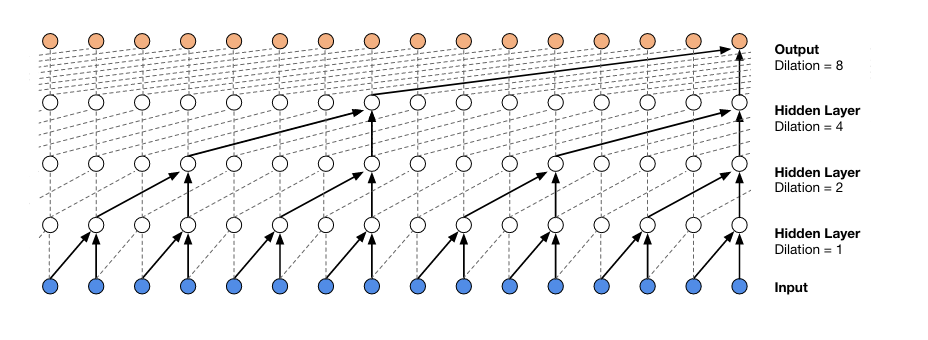
\includegraphics[width=\textwidth]{figures/2-sota/dilated-convolution.png}
    \caption[WaveNet]{\textbf{WaveNet} --- This illustration was taken from \cite{oord_wavenet_2016}. It shows the idea behind WaveNet, applying dilated convolutions to \ac{AR} models.}
    \label{fig:dilated-convolution}
\end{figure}

This structure enables WaveNet to capture long-range dependencies in the input sequence, which is crucial for generating high-quality audio. If an \ac{RNN} (see Section \ref{sec:rnn}) sees only one input sample at each time step, WaveNet has direct access to multiple input samples \cite{huzaifah_deep_2021}. For example, in speech generation, WaveNet can use its sizeable receptive field to model the relationship between a word spoken early in a sentence and its pronunciation later in the sentence.

WaveNet uses a softmax activation function at each output node to produce a probability distribution over the possible values at each time step. During training, the network is fed sequences of input data and their corresponding ground truth values. The model's parameters are adjusted so that its outputs match the ground truth as closely as possible.

WaveNet can use its trained parameters to generate new sequences by sampling from its output probability distribution during generation. This allows it to generate diverse and high-quality outputs, such as realistic human speech or written text, by combining its learned representations of the underlying data distribution with a small amount of randomness.

The input of WaveNet is usually a Mel-Spectrogram (or other representations), and the output is the sound signal.

WaveNet can be conditioned on, for instance, text for \ac{TTS} settings by feeding extra information about the text itself (\textit{e.g.} embeddings). If a model is not conditioned on text, it generates random sounds without any global structure behind it.

The results were astonishing. ``A single WaveNet can capture the characteristics of many different speakers with equal fidelity, and can switch between them by conditioning on the speaker identity. When trained to model music, we find that it generates novel and often highly realistic musical fragments.'' \cite{oord_wavenet_2016}.

Even though this model is good at learning the characteristics of sounds over brief periods, it struggles with global latent structure. They are also very slow for training and inferring \cite{tahiroglu_-terity_2020}.

%%%%%%%%%%%%%%%%%%%%%%%%%%%%%%%%%

\subsubsection{WaveNet Variants} \label{sec:wavenet-variants}

The WaveNet model has emerged as a powerful tool for generating high-quality audio waveforms, particularly for speech and music applications. However, its architecture, which employs dilated convolutions and deep residual networks, can be computationally intensive and challenging to train. To address these limitations, several WaveNet variants have been proposed in recent years that aim to reduce the complexity of the model while maintaining its effectiveness.

One such variant is \textbf{WaveRNN} \cite{kalchbrenner_efficient_2018}, which employs a single \ac{RNN} (see Section \ref{sec:rnn}) to approximate the dilated convolutions in WaveNet. This approach significantly speeds up training time while maintaining the quality of the generated audio. Another variant, FloWaveNet \cite{kim_flowavenet_2018}, employs a flow-based generative model (Section \ref{sec:flow-model}) that allows for efficient training with only one training stage while producing high-quality audio. Additionally, Fast WaveNet  \cite{paine_fast_2016} employs a caching mechanism to reduce the computational cost of the model while maintaining an \ac{AR} structure.

These WaveNet variants are unique in their architectures and training procedures but share the goal of making audio generation more efficient and accessible. While these models are primarily focused on speech and music generation, they can be adapted to other types of audio data. Ongoing research in this area may explore further optimization of these models, integration with other models, and application to new domains.

\subsubsection{MelGAN} \label{sec:melgan}

According to Kumar et al. in 2019, in their \textit{MelGAN} paper~\cite{kumar_melgan_2019}, audio generation with \acp{GAN} is possible although a challenging task (see Section \ref{sec:gan}). Previous studies in this field have encountered difficulties generating coherent raw audio waveforms using \acp{GAN}. Nonetheless, Kumar et al. demonstrate in their \textit{MelGAN} paper that introducing certain architectural changes makes it feasible to train \acp{GAN} to generate high-quality and coherent audio waveforms reliably.

The generator of MelGAN is a fully convolutional feed-forward network that takes a Mel-Spectrogram as input and generates a raw waveform as output. This approach allows for efficient and parallelized processing of audio data.

The decoder takes the waveform and decides whether it is a realistic sound. The decoder is not a single neural network but a multi-scale architecture with three discriminators (D1, D2, D3). These discriminators have identical network structures but operate on different audio scales. D1 operates on the scale of raw audio, while D2 and D3 operate on raw audio downsampled by a factor of 2 and 4, respectively. The use of multiple discriminators at different scales is motivated by the fact that audio has structure at different levels.

MelGAN proved itself way faster than other architectures such as WaveNet (see Section \ref{sec:wavenet}) with comparable results (for inference, roughly thirty-six thousand times faster than WaveNet), given its reduced number of parameters.


%%%%%%%%%%%%%%%%%%%%%%%%%%%%%%%%%

\subsubsection{GANSynth} \label{sec:gansynth}

\textit{GanSynth}, presented in 2019, \cite{engel_gansynth_2019} is a \ac{GAN} (see Section \ref{sec:gan}) that uses log-magnitude spectrograms and phases to generate coherent waveforms. Compared to directly generating waveforms with stridden convolutions, the use of spectrograms and phases has been shown to produce better results.

The study focuses on the NSynth \cite{engel_neural_2017} dataset, a collection of 300 000 musical notes from 1 000 different instruments.

The model first samples a random vector $z$ from a spherical Gaussian distribution. This vector is passed through a stack of transposed convolutions, which upsample and generate output data $x = G(z)$. This generated data is then fed into a discriminator network, which uses downsampling convolutions to estimate a divergence measure between the real and generated distributions.

The architecture of the discriminator network mirrors that of the generator, which allows for a more efficient training process. Optimizing the divergence measure allows the generator to produce spectrograms and phases that resemble actual musical notes more closely.

The study results demonstrate that \acp{GAN} outperform WaveNet (see Section \ref{sec:wavenet}) baselines on automated and human evaluation metrics and can efficiently generate several audio orders of magnitude faster than their \ac{AR} counterparts.

%%%%%%%%%%%%%%%%%%%%%%%%%%%%%%%%%

\subsubsection{HiFi-GAN}

Proposed in 2020, \textit{HiFi-GAN} \cite{kong_hifi-gan_2020} is a \ac{GAN} (see Section \ref{sec:gan}) model that combines efficiency and high-fidelity speech synthesis. HiFi-GAN achieves this by leveraging the periodic patterns inherent in speech audio, demonstrating that modeling these patterns is crucial for enhancing sample quality. The model includes a generator and two discriminators, trained adversarially, and two additional losses for improving training stability and model performance.

The generator is a fully \ac{CNN} (see Section~\ref{sec:CNN}) that takes Mel-Spectrograms as input and upsamples them through transposed convolutions, matching the temporal resolution of raw waveforms. The discriminators are the \ac{MSD} and a \ac{MPD}. \Ac{MSD} evaluates the audio sequence on different scales using a mixture of three convolutional sub-discriminators with different average pools. At the same time, \ac{MPD} consists of small sub-discriminators that capture different implicit structures of input audio by looking at different parts, accepting only equally spaced samples of input audio with different periods. 

HiFi-GAN's performance is evaluated using a subjective human evaluation (\ac{MOS}) on a single speaker dataset, which shows that the proposed method exhibits similarity to human quality. The model achieves a higher \ac{MOS} score than WaveNet (see Section \ref{sec:wavenet}).

Importantly, HiFi-GAN achieves this high-quality synthesis efficiently. Specifically, the model generates 22.05 kHz high-fidelity audio 167.9 times faster than real-time on a single V100 \ac{GPU}, demonstrating superior computational efficiency compared to AR and flow-based models. Moreover, a small-footprint version of HiFi-GAN generates samples 13.4 times faster than real-time on \ac{CPU} with comparable quality to an \ac{AR} counterpart.

\subsection{End-to-End Models} \label{sec:end-to-end}

Audio synthesis is the task of producing artificial audio from text or other kinds of data. Traditionally, audio synthesis systems consist of multiple stages, such as a data analysis frontend, a sound model, and an audio synthesis module. Building these components requires extensive domain expertise and may contain brittle design choices. Moreover, these components are usually trained separately on different objectives and datasets, which may introduce errors and inconsistencies in the final output. To overcome these limitations, end-to-end models have been proposed that directly learn the mapping between text (or other kinds of data) and audio waveform using deep neural networks. These models are presented in this Section.

Existing research establishes two main frameworks for end-to-end models: specialized models designed for a specific domain, and universal models aimed at broader applications. The table \ref{tab:end-to-end-audio-models} shows some examples of these models based on their type, input, output, model architecture, and type of conditioning. Specialized models target either speech or music synthesis, such as Char2wav and Jukebox. Researchers have developed different subsets of technologies within speech and music synthesis models, such as neural codec speech models and discrete diffusion models. Universal models, such as SampleRNN and AudioGen, can generate audio from various inputs and domains, such as text or raw audio seeds.

\begin{table}[ht]
\centering
\caption{A comparison of different end-to-end generative models for audio.}
\begin{tabularx}{\textwidth}{|l|l|X|X|X|}
\hline
\textbf{Model} & \textbf{Type} & \textbf{Input}            & \textbf{Output}                        & \textbf{Model Architecture}                                                      \\ \hline
Char2wav~\cite{sotelo_char2wav_2017}       & Speech        & Text prompt               & Raw audio waveform                     & Encoder-decoder with attention and neural vocoder                                \\ \hline
VALL-E~\cite{wang_neural_2023}         & Speech        & Text and acoustic prompt  & Raw audio waveform                     & Neural codec language model and neural vocoder                                   \\ \hline
Jukebox~\cite{dhariwal_jukebox_2020}        & Music         & Genre, artist, and lyrics & Raw audio waveform                     & Hierarchical VQ-VAE and autoregressive Transformer                               \\ \hline
Riffusion~\cite{forsgren_riffusion_2022}      & Music         & Text prompt               & Raw audio waveform                     & Neural codec language model based on discrete diffusion model and neural vocoder \\ \hline
MusicLM~\cite{agostinelli_musiclm_2023}        & Music         & Text prompt               & Raw audio waveform                     & Neural codec language model and neural vocoder                                   \\ \hline
SampleRNN~\cite{mehri_samplernn_2017}      & General       & None                      & Raw audio waveform                     & Hierarchical RNN and neural vocoder                                              \\ \hline
AudioLM~\cite{borsos_audiolm_2022}        & General       & Text prompt               & Raw audio waveform                     & Hybrid tokenization scheme with Transformer models and neural vocoder            \\ \hline
DiffSound~\cite{yang_diffsound_2022}      & General       & Text prompt               & Mel-spectrogram and raw audio waveform & VQ-VAE, discrete diffusion model, and neural vocoder                             \\ \hline
AudioGen~\cite{kreuk_audiogen_2023}       & General       & Text prompt               & Mel-spectrogram and raw audio waveform & Transformer-based generative model and neural vocoder                            \\ \hline
\end{tabularx}
\label{tab:end-to-end-audio-models}
\end{table}

%%%%%%%%%%%%%%%%%%%%%%%%%%%%%%%%%

\subsubsection{Text-to-Speech} \label{sec:tts}

\Acf{TTS} models are designed to convert written text into synthesized speech. These models use deep neural networks to directly learn the mapping between written text and audio waveform. Leveraging developments in \ac{NLP} and speech synthesis techniques, \ac{TTS} models have made significant progress in generating high-quality, human-like speech from text input. This Section examines some of the notable \ac{TTS} models that have been developed recently.

\input{src/chapters/2-state-of-the-art/related-work/end-to-end/char2wav}
\input{src/chapters/2-state-of-the-art/related-work/end-to-end/vall-e}

\subsubsection{Generative Music}

Generative music is created using generative techniques. End-to-end generative music models enable the production of new musical compositions without using predefined templates or samples, directly from textual or other data inputs. These models use \ac{DL} architectures to capture patterns and structures within different genres or styles of music, and can produce original pieces based on given prompts. This Section explores remarkable generative music models that demonstrate their ability to compose novel musical arrangements.

\input{src/chapters/2-state-of-the-art/related-work/end-to-end/jukebox}
\input{src/chapters/2-state-of-the-art/related-work/end-to-end/riffusion}
\input{src/chapters/2-state-of-the-art/related-work/end-to-end/musiclm}

\subsubsection{General Text-to-Audio}

Text-to-audio systems have a wide range of applications beyond speech synthesis or generative music tasks. End-to-end models convert different forms of textual input into corresponding audio outputs. The outputs have diverse purposes, including sound effects generation, voice transformation, and environmental sound synthesis. These models provide flexible solutions for transforming text into realistic auditory experiences by training on large-scale datasets containing paired text-audio examples across various domains. This Section presents several text-to-audio approaches that demonstrate innovative methods of audio synthesis based on specific textual cues.

\input{src/chapters/2-state-of-the-art/related-work/end-to-end/samplernn}
\input{src/chapters/2-state-of-the-art/related-work/end-to-end/audiolm}
\input{src/chapters/2-state-of-the-art/related-work/end-to-end/diffsound}
\input{src/chapters/2-state-of-the-art/related-work/end-to-end/audiogen}



% TODO: pick a name according to the domain
\chapter{Problem}\label{chap:problem}
% TODO: pick a name according to the domain

% TODO
audio is 1-D data.\cite{oord_wavenet_2016}

raw audio is typically stored as a sequence of 16-bit integer values (one per timestep). \cite{oord_wavenet_2016}
% TODO: pick a name according to the domain
\chapter{Development and Implementation} \label{chap:solution}

\minitoc

This thesis's development and implementation chapter corresponds to the crucial task of developing the solution. This chapter comprehensively explores the methodology, dataset analysis, generative model development, and research plan. This chapter aims to provide a detailed account of the steps taken to achieve the research objectives and contribute to the field of generative AI models for audio.

In Section~\ref{sec:sol-approach}, the author outlines the approach taken in developing this thesis. Section~\ref{sec:sol-datasets} details the various datasets considered in this research. A thorough description and analysis of these datasets is provided, highlighting their characteristics and potential challenges. 

Section~\ref{sec:sol-models} forms the core of this research. There, the author presents the development of several generative models, including the central model, GANmix. The model architecture, training process, and evaluation are discussed, demonstrating their contributions to the field and their potential for generating audio samples.

In addition, Section~\ref{sec:work-plan} outlines the timeline for the development of this thesis. A roadmap of key milestones and stages is provided.

Finally, practical information and resources, such as the source code, are available at \url{https://ctrlmarcio.github.io/audio-gen-ai/}. This allows interested readers to access and explore the codebase, facilitating further research and collaboration.

\section{Methodology and Approach} \label{sec:sol-approach}
 
The development of this dissertation is divided into three main parts:

\begin{itemize}
    \item The state-of-the-art research;
    \item The development;
    \item The writing of the document;
\end{itemize}
 
These areas were not necessarily exclusive. That is, they overlapped. Initially, work began with general research into the state of the art in modeling and audio processing. Early development began after establishing a basic understanding of what needed to be achieved. This development took place in parallel with the ongoing research. As issues arose during development, additional research was required to address them. Writing the document was an ongoing process that led to clearer thinking and planning. Nevertheless, writing was prioritized after the bulk of the development was complete.

The interaction between these phases is both dynamic and symbiotic. The state-of-the-art research phase is the foundation, providing information for future model development decisions. Research insights directly influence the design and direction of generative models. As development progressed, new challenges and possibilities emerged, triggering further exploration in the state-of-the-art literature. Similarly, the development phase provides empirical insights that contribute to refining the writing process. Model development findings and outcomes contribute to comprehensive and informative document content. This iterative interplay ensures that each phase informs, enriches, and refines the others, leading to a coherent and impactful dissertation.

\subsection{State-of-the-Art Research}

One of the goals of this thesis is to provide a comprehensive overview of the current state-of-the-art audio synthesis through textual input. A systematic and thorough approach was taken to search and review the relevant literature.

The process started with the collection of keywords related to the topic of audio synthesis and generative \ac{AI} models. Through multiple combinations, these keywords were then used to search multiple online sources, including academic search engines such as Google Scholar and the Universidade do Porto's. Searches were also conducted for specific papers given the author's knowledge. The results of these searches were analyzed to identify publications with significant citations and high relevance to the thesis topic.

These publications were then carefully read and analyzed, and their citations were further investigated to expand the search and deepen the understanding of the state-of-the-art in the field. If any aspect of a publication was unclear, additional research was conducted to clarify the concept and find additional relevant literature.
This process of searching, reading, and analyzing was iterated multiple times, allowing the gathering of new keywords and publications. Notes and possible citations for each publication were stored in a private database, allowing easy access and organization.

\subsection{Model Development} \label{sec:problem-model-development}

The development of audio synthesis models is a progressive approach that aims to achieve three primary objectives. Together, these goals guide the development of the models and ensure a comprehensive exploration of audio synthesis through text.

The primary objective is establishing fundamental models that facilitate an in-depth understanding of sound representation and \ac{DL} principles. To achieve this, the initial focus was on tasks like audio classification. These fundamental models are developed using smaller datasets like Audio MNIST~\cite{becker_interpreting_2018}. This step provides a foundational grasp of the models' capabilities and acts as a basis for subsequent progress.

The second goal is to develop generative models to synthesize audio from textual input. These generative models are designed to create audio content that aligns with provided text prompts by building on the insights gained from fundamental models. The progressive approach provides the ability for the generative process's iterative refinement, optimization, and enhancement.

The third goal includes proposing theoretical models that establish the foundation for more advanced generative techniques. Although not all theoretical approaches are entirely implemented, these concepts add to the broader discussion of audio synthesis research. Exploring theoretical models boosts innovation and promotes the development of new strategies for generating audio from text.

The model development approach provides an exhaustive and iterative pathway to achieve an effective and innovative audio synthesis from textual input by pursuing these interconnected objectives.

\subsection{Writing of the Dissertation}

This dissertation was composed with a focus on clarity, conciseness, and informative content. A continuous approach was utilized to achieve this objective, consisting of three key phases for each section: initial drafting, incorporation of researched references, and ongoing refinement. This iterative process required multiple re-readings and revisions. This dynamic method aligns well with the principles of agile development~\cite{dingsoyr_decade_2012}, promoting flexibility and continuous progress during the writing process.

Furthermore, this document adheres to established academic norms, encompassing writing style, citational methodologies, and the lucid and consistent presentation of results and figures. In addition to the individual author's contributions, the insights of the thesis coordinators have strengthened this project. They have diligently reviewed and enhanced the document to ensure its precision and authenticity.

This dissertation, crafted with meticulous attention to detail, linguistic technologies, and rigor and scrutiny, is the culminating embodiment of the author's resolute research pursuits and the zenith of scholarly achievement.
\section{Dataset Selection and Analysis} \label{sec:sol-datasets}

This section is crucial to synthesizing audio from text inputs, as it reveals the foundation on which the generative models are developed and improved. Datasets are the foundation of this research. These datasets serve as the learning material for \ac{DL} algorithms and a means to evaluate the perceptual quality, coherence, and creativity of the resulting audio outputs.

It presents the datasets researched and used to implement the models. It is worth noting that datasets that are well-known within the field but are neither used nor relevant to the specific problem at hand, are excluded from citation. For example, this discussion does not include datasets specialized in speech or music. In addition, although the data size is significant for \ac{DL} algorithms, all the datasets discussed in this section include more than 1000 sound samples. Nonetheless, it is important to recognize that this number is relatively small compared to image recognition datasets with millions of entries, like CLIP~\cite{radford_learning_2021}, commonly used in the field.

Two types of datasets are cataloged, differentiated mostly by the nature of the adopted label – \emph{categorical} and \emph{descriptive}. A categorical-label dataset comprises sounds that are associated with a single, distinct label, such as ``music'', ``piano'', or ``singing''. On the other hand, descriptive-label datasets comprise natural language sentences or textual descriptions of soundscapes, such as  ``boy singing while playing the piano''. In the realm of \ac{DL}, descriptive-labeled datasets are deemed more conducive. Nevertheless, datasets containing categorical labels can still be valuable when undergoing augmentation techniques. To the author's knowledge, Table~\ref{tab:datasets} provides a comprehensive list of audio datasets that meet the aforementioned criteria to date.


\begin{table}[ht]
\centering
\caption{Comparison of datasets for soundscapes}
\label{tab:datasets}
\begin{tabularx}{\textwidth}{|X|X|X|X|X|}
\hline
\textbf{Name} &
  \textbf{Type} &
  \textbf{\# Samples} &
  \textbf{Duration} &
  \textbf{Labels} \\ \hline

Acoustic Event Dataset \cite{takahashi_deep_2016} &
  Categorical labeled &
  5223 &
  Average 8.8s &
  One of 28 labels \\ \hline

AudioCaps \cite{kim_audiocaps_2019} &
  Descriptive labeled &
  39597 &
  10s each &
  9 words per caption \\ \hline

AudioSet \cite{gemmeke_audio_2017} &
  Categorical labeled &
  2084320 &
  Average 10s &
  One or more of 527 labels \\ \hline

Audio MNIST~\cite{becker_interpreting_2018}&
  Categorical labeled &
  30000 &
  Average 0.6s &
  One of 10 labels \\ \hline
  
Clotho \cite{drossos_clotho_2019} &
    Descriptive labeled &
    4981 &
    15 to 30s &
    24 905 captions (5 per audio). 8 to 20 words long each \\ \hline
    
FSDKaggle2018 \cite{fonseca_general-purpose_2018} &
  Categorical labeled &
  11073 &
  From 300ms to 30s &
  One or more of 41 labels \\ \hline
  
UrbanSound8K \cite{salamon_dataset_2014} &
  Categorical labeled &
  8732 &
  Less or equal to 4s &
  One of 10 labels \\ \hline
  
YouTube-8M Segments \cite{abu-el-haija_youtube-8m_2016} &
  Categorical labeled &
  237000 &
  5s &
  One or more of 1000 labels \\ \hline
\end{tabularx}
\end{table}

\subsection{Categorical Labeled Datasets}

The datasets represented here are the ones where the audio samples are tagged with simple labels. An example of one of these labels might be ``Dog''. This labeling contrasts complete with descriptive labeling as seen in Section~\ref{sec:sound-nl-labelled}. Even though these datasets are not perfect for this use case, they might be augmented or enhanced (see Section~\ref{sec:text-augmentation}). One such example would be taping different sounds. For instance, taping a ``dog''  ``bark'' with a ``truck'' ``honk'' could generate the label ``a dog barking followed by a truck honking''.

The datasets presented here contain audio samples tagged with simple labels such as ``Dog'', in contrast to the descriptive labeling discussed in Section~\ref{sec:sound-nl-labelled}. While these datasets may not be ideal for the purposes of this thesis, they can be augmented or enhanced (as explained in Section~\ref{sec:text-augmentation}) through means such as taping difference sounds. For example, joining a ``do barking'' and a ``truck honking'' could produce the label ``a dog barking followed by a truck honking.''


\subsubsection{Acoustic Event Dataset}

Information regarding this dataset is not much, and the classes have rather specific names such as ``hammer'' or ``mouse\_click''. Nevertheless, it has 5223 samples, completing 768.4 minutes, representing 28 different classes \cite{takahashi_deep_2016}.

\subsubsection{Audio MNIST} \label{sec:dataset-amnist}

Audio MNIST \cite{becker_interpreting_2018} is a sonic take on the famous MNIST dataset \cite{deng_mnist_2012}. It has a series of 60 speakers saying different numbers from 0 to 9. These samples add up to 30000 samples.

This dataset is not used in the model but rather as a first take for every baseline model for its simplicity and small size.

\subsubsection{AudioSet}

AudioSet is the most comprehensive dataset existent for audio \cite{gemmeke_audio_2017}.

It is a large-scale, high-quality dataset of annotated audio clips. It was created by Google Research and released in 2017 as part of the ongoing effort to advance state-of-the-art audio understanding.
The dataset consists of over 2 million 10-second audio clips, each annotated with one or more labels from a set of 527 classes, covering a wide range of sounds such as human speech, animal vocalizations, musical instruments, environmental sounds, and more. The audio clips are sourced from YouTube videos and cover diverse content, including news broadcasts, movie trailers, music videos, and everyday videos.

The annotations in AudioSet are created using a hierarchical ontology, where the classes are organized into a tree-like structure based on their semantic relationship. This allows for a more fine-grained representation of audio events and makes it easier for machine learning models to learn the relationship between different sound categories.

\subsubsection{FSDKaggle2018}

Freesound Dataset Kaggle 2018 \cite{fonseca_general-purpose_2018} is an audio dataset containing 11,073 audio files annotated with 41 labels following the same ontology as AudioSet. The sounds were taken from Freesound which is an online database maintained by the community. So, the quality may vary.

This dataset was used for competitions on Kaggle regarding sound classification.

\subsubsection{UrbanSound8K}

The UrbanSound8K \cite{salamon_dataset_2014} is an available dataset focusing on urban sounds. It is one of the largest and most diverse datasets of its kind.

The UrbanSound8K dataset consists of 8732 audio clips, each lasting approximately 4 seconds, collected from various urban environments. The audio clips are annotated with one of 10 classes. The classes in the dataset represent a wide range of typical urban sounds.
The audio clips in the UrbanSound8K dataset are collected from various sources, including YouTube and Freesound, and are carefully selected to ensure a diverse and representative sample of urban sounds. The dataset includes audio recordings from different cities, captured in different seasons and weather conditions, to provide a wide range of sound characteristics and environments.

\subsubsection{YouTube-8M Segments}

The YouTube-8M Dataset is a significant video dataset \cite{abu-el-haija_youtube-8m_2016} that contains millions of YouTube video IDs with high-quality machine-generated annotations from a diverse vocabulary of over 3,800 visual entities. This dataset aims to accelerate research on large-scale video understanding, representation learning, noisy data modeling, transfer learning, and domain adaptation approaches for video.

Upon reviewing the YouTube-8M dataset, it is evident that the minimum video length constraint of 120 seconds makes it unsuitable for this research as it should focus on snippets shorter than this length.

An alternative dataset that may suit this research's needs is the YouTube-8M Segments Dataset. This dataset is an extension of the YouTube-8M dataset and comes with human-verified segment annotations that temporally localize entities in videos. With about 237K human-verified segment labels on 1000 classes, the dataset enables the training of models for temporal localization using a large amount of noisy video-level labels in the training set.

The vocabulary of the segment-level dataset is a subset of the YouTube-8M dataset vocabulary, excluding entities that are not temporally localizable, such as movies or TV series that usually occur in the whole video. The dataset also provides time-localized frame-level features, enabling classifier predictions at the segment-level granularity.

While the YouTube-8M Segments Dataset provides temporal annotations for video entities, this dataset could still be valuable if one extracts the audio from each YouTube video, as it includes time-localized frame-level features that could be used for audio analysis. Thus, while the video content may not be essential for this research project, the YouTube-8M Segments Dataset could still be a valuable audio-analysis resource.

\subsection{Descriptive Labeled Datasets} \label{sec:sound-nl-labelled}

The datasets presented here present way richer textual information regarding the sound. For instance, instead of a sound being connected with the label ``engine'', datasets in this section connect it with a sentence such as ``a vehicle engine revving''. This allows for training the natural language input, one of the main assumed problems.

\subsubsection{AudioCaps}

AudioCaps \cite{kim_audiocaps_2019} is a large-scale dataset of 46 thousand audio clips with human-written text pairs collected via crowdsourcing on the AudioSet dataset.

\subsubsection{Clotho Dataset} \label{sec:clotho}

Clotho \cite{drossos_clotho_2019} is an audio dataset that consists of 4981 audio samples. Each audio sample has five captions (a total of 24 905 captions). Audio samples are 15 to 30 seconds long, and captions are 8 to 20 words long. 

A practical example is a sound that is described both by ``a car honks from the midst of a rainstorm'', ``rain from a rainstorm is hitting surfaces and a car honks'', and others.
\section{Generative Model Development} \label{sec:sol-models}

Audio synthesis is the process of creating artificial sounds from scratch. It is a challenging task that requires a deep understanding of the nature and structure of sound, as well as the ability to generate realistic and diverse audio samples. Generative models have been widely used in image synthesis, but their application to audio synthesis is relatively new and less explored.

This section presents the development of a novel generative model for audio synthesis, called GANmix, which combines elements of both a \ac{GAN} and a \ac{VAE}. GANmix exploits the strengths of both models to produce high-quality and diverse audio samples in a computationally efficient manner. GANmix also allows for latent space manipulation, which can be used to control various aspects of the generated audio, such as pitch, timbre, and style.

Before introducing GANmix, this section also describes a series of exploratory experiments that provide a valuable learning phase for the development of the main model. The experiments cover different aspects of audio synthesis, such as audio representation, model architecture, training process, dataset, and evaluation metrics. The experiments aim to provide insight into the performance, limitations, and potential of different generative audio models.

The section is organized as follows: Section~\ref{sec:findings} presents the exploratory experiments that inform the development of GANmix. Section~\ref{sec:ganmix} introduces GANmix as a novel technique for audio synthesis. 

\subsection{Exploratory Experiments} \label{sec:findings}

In the development of generative \ac{AI} models for audio synthesis, it is crucial to conduct extensive experiments that explore various aspects of model architecture, training processes, datasets, and evaluation metrics. This section presents a series of experiments that provide a valuable learning phase before developing the primary model, GANmix. The experiments aim to gain insight into the performance, limitations, and potential of different generative audio models. The author analyzes empirical findings to inform the development of GANmix, aiming for a robust and efficient solution.

The initial experiment focuses on a classification model to uncover the fundamental principles of sound. Training the model on labeled audio data, the author aims to grasp the connections among different audio features and their corresponding categories. This experiment lays the foundation for further research on audio representation.

Based on the results of the classification experiment, the author proceeds to develop a \ac{GAN} for audio synthesis. The aim of this study is to assess the effectiveness of \acp{GAN} in generating high-quality and realistic audio samples.

Furthermore, the author explores the efficacy of \acp{AE} and \acp{VAE} in audio generation. The experiments investigate the reconstruction and generation capabilities of these models, respectively.

The purpose of these experiments is to achieve a comprehensive understanding of both audio and different generative models for audio synthesis. These empirical findings provide a crucial basis for developing GANmix, ensuring a robust and effective solution for audio generation.

\include{src/chapters/4-solution/models/empirical/1-classification}
\include{src/chapters/4-solution/models/empirical/2-gan}
\include{src/chapters/4-solution/models/empirical/3-autoencoder}
\include{src/chapters/4-solution/models/empirical/4-vae}
\subsection{GANmix} \label{sec:ganmix}

This section introduces GANmix as a novel technique for audio generation that fuses components of both a \ac{GAN} and a \ac{VAE}. GANmix addresses the problem of generating high-quality audio under resource constraints.

Audio generation is computationally expensive, especially when constrained by hardware capabilities. GANmix offers a potential solution by combining the strengths of \acp{GAN} and \acp{VAE} to improve audio synthesis in limited computational environments through latent space manipulation.

\paragraph{Model Architecture Plan}

The GANmix architecture consists of a generator and a discriminator that operate in latent space rather than in the space of the sound or soundscape. This approach was inspired by stable diffusion (see Section~\ref{sec:stable-diffusion}), which generates samples through its latent space instead of working on the sample space itself.

Traditionally, in \acp{GAN}, the generator produces samples to be evaluated by the discriminator. However, GANmix takes a different approach: its generator produces values in an embedding space defined by the pre-trained AudioLDM \ac{VAE} encoder~\cite{liu_audioldm_2023}. The discriminator, on the other hand, objectively verifies latent features by comparing the generated features with those obtained by the \ac{VAE} encoder. Samples are generated posteriorly by passing the generated features through the decoder of the \ac{VAE}.

The decision to incorporate the AudioLDM \ac{VAE} model within the GANmix architecture was based on thoughtful reasons.

\begin{enumerate}
    \item \textbf{\ac{VAE} Training:} Training \acp{VAE} poses a challenge since it typically requires significant computational resources and extensive datasets to achieve effective convergence. Previous experiences with model development (in Section~\ref{sec:training-vae}) for this thesis highlighted the intricacies involved in \ac{VAE} training.
    \item \textbf{AudioLDM's High-Performance:} At the time of GANmix's development, the AudioLDM model was one of the top models for audio generation.
    \item \textbf{Accessibility and Open Source Nature of AudioLDM:} One key benefit of integrating the AudioLDM \ac{VAE} model into GANmix architecture was its openness and accessibility through platforms like Hugging Face's model hub through \url{https://huggingface.co/cvssp/audioldm}. This accessibility streamlined the incorporation of the high-performing AudioLDM.
\end{enumerate}

The generator is designed to convert random Gaussian noise vectors into latent features that resemble the encodings of the AudioLDM \ac{VAE} model. Initially, a convolutional model was designed. It used four convolutional transpose 2D layer blocks, with Leaky \ac{ReLU} activation functions following three of them. Each block comprised several convolutional layers. Furthermore, after the deconvolutional layer, two convolutional layers are employed to preserve the data's shape. The final block, responsible for producing the transformed audio samples, did not use an activation function. This design decision enabled the generator to generate unrestricted values, ensuring the accuracy of the produced audio samples.

The decision to utilize 2D convolutions arised from the innate characteristics of the latent features generated by the AudioLDM \ac{VAE} model. These latent features have various dimensions, and integrating 2D convolutional layers enabled GANmix to efficiently grasp complicated patterns across these dimensions. By utilizing 2D convolutions, the architecture could more effectively utilize the multidimensional information in the latent representations, resulting in an improved quality of the generated audio output.

The discriminator architecture mimicked that of the generator with three blocks of convolutional 2D layers using leaky \ac{ReLU} activation. Each block contained multiple convolutional layers (three in the proposed architecture). The final layer of the discriminator applied a sigmoid activation function to generate a probability score indicating the authenticity of the input audio sample.

\paragraph{Experimental Results}

Preliminary experiments with GANmix and the Audio MNIST dataset produced promising but flawed results. Objective analysis reveals that the generator's performance lagged behind the discriminator's, resulting in suboptimal sample quality. Therefore, the training process requires further refinement.

In order to bridge the performance gap between generator and discriminator, a range of refinements were explored. These efforts included exploring different optimizers, such as Adam, RMSProp, and SGD (see Section~\ref{sec:dl-foundations}), each with varying hyperparameters. In addition, the author adjusted model sizes, experimented with diverse loss functions, and introduced noise to training samples. However, the speed of training and comprehensive experimentation were still hindered by hardware resource limitations.

More information regarding these explorations can be found in Chapter~\ref{chap:results}.

With access to a more powerful computing environment, GANmix was further developed using the Clotho dataset (see Section~\ref{sec:clotho}), leading to a significant improvement in the quality of generated audio samples. Nonetheless, there were still issues with achieving equilibrium between the generator and discriminator, even with the upgraded dataset.

\paragraph{Final Model}

After conducting a series of experiments, the GANmix model reached its culmination. This architecture incorporates the Clotho dataset and includes significant improvements to both the generator and discriminator.

The GANmix model is the final model used in this thesis, corresponding to the model used in Experiment 10. Unlike most state-of-the-art generative models that use \acp{CNN}, the GANmix model uses fully connected neural networks for both the generator and the discriminator. The rationale for this was empirical and is given in section~\ref{sec:exp10}.

The generator takes as input a random Gaussian noise vector of size $NZ$ and passes it through a fully connected hidden layer of $NH$ neurons. The output of the hidden layer is then fully connected to another layer of size $EW \times EH \times ED$, where $EW$, $EH$, and $ED$ are the width, height, and number of dimensions of the embeddings generated by the \ac{VAE}, respectively. The output layer is reshaped to match the shape of the \ac{VAE} embeddings.

The discriminator takes as input an embedding of shape $EW \times EH \times ED$ and flattens it to a vector. The vector is then passed through a fully connected hidden layer of $NH$ neurons, and then fully connected to a single output neuron that applies a tanh activation function.

The \ac{VAE} encoder and decoder are pre-trained by a state-of-the-art network, AudioLDM. However, the GANmix model can work with any \ac{VAE} network, as long as the size of the last layer of the generator (and the first layer of the discriminator) is adjusted accordingly.

The loss function used to train the GANmix model is \ac{BCE}. The generator is optimized using Adam with a learning rate of $1 \times 10^{-3}$, while the discriminator is optimized using Adam with a learning rate of $1 \times 10^{-4}$. A scheduler updates the learning rate every 10 epochs.

The implementation of GANmix can be found in Appendix~\ref{ann:ganmix-implementation}. More about the configuration and parameters of the GANmix model can be found in Appendix~\ref{ann:ganmix-conf}. The model's architecture is shown in Figure~\ref{fig:ganmix-architecture}.

\begin{figure}[ht]
    \centering
    \includegraphics[width=\textwidth]{figures/4-solution/ganmix.pdf}
    \caption[GANmix architecture]{\textbf{GANmix architecture} --- On the left is the GANmix generator with three layers: the initial noise layer with $NZ$ neurons, the hidden layer with $NH$ neurons, and the layer corresponding to the embedding space with $EW \times EH \times ED$ neurons. The outputs of this layer are transformed into the form of the outputs of the \ac{VAE}. On the right is the discriminator that mirrors the generator. The last layer has a single neuron with a sigmoid activation function. At the top is a spectrogram that passes through the pre-trained \ac{VAE} generator to generate the latent space. At the bottom, the opposite happens: embeddings in the latent space go through the \ac{VAE} decoder to generate the audio sample in the form of a spectrogram.}
    \label{fig:ganmix-architecture}
\end{figure}

\section{Research Plan} \label{sec:work-plan}

% The work plan refers to the specific tasks and activities that will be carried out in order to execute the approach

% The work plan, on the other hand, is a more detailed plan that outlines the specific tasks and activities that will be carried out in order to implement the approach. This might include tasks such as data collection, data analysis, and the development of any necessary software or tools. The work plan should also include a timeline for completing these tasks and any milestones that need to be achieved along the way.

% the work plan should be described in more detail in the later stages of the project, as the research progresses and the specific tasks and activities become clearer.

\begin{figure}[ht]
    \centering
    \begin{ganttchart}[
            time slot format=isodate,
            expand chart=\textwidth,
            title/.style={draw=none, fill=none},
            bar label node/.append style={align=right},
        ]{2022-09-01}{2023-08-31}
        \gantttitlecalendar{year, month} \\
        
        \ganttbar[bar/.append style={fill=input, draw=none}]{State-of-the-Art}{2022-09-01}{2023-02-15} \\
                    
        \ganttbar[bar/.append style={fill=output, draw=none}]{Introduction}{2022-10-01}{2022-12-31} \\
                    
        \ganttbar[bar/.append style={fill=input, draw=none}]{Gather of Dataset}{2022-11-01}{2023-05-31} \\
        
        \ganttbar[bar/.append style={fill=output, draw=none}]{Defining the Problem}{2022-11-15}{2022-12-15} \\
        
        \ganttbar[bar/.append style={fill=neuron, draw=none}]{Basic Classification}{2023-03-01}{2023-03-31} \\
                    
        \ganttlinkedbar[bar/.append style={fill=neuron, draw=none}]{Basic Generation}{2023-04-01}{2023-05-31} \\
                    
        \ganttlinkedbar[bar/.append style={fill=neuron, draw=none}]{Apply Large Datasets}{2023-06-01}{2023-06-30} \\

        \ganttlinkedbar[bar/.append style={fill=neuron, draw=none}]{Collect Results}{2023-07-01}{2023-08-14} \\

        \ganttbar[bar/.append style={fill=output, draw=none}]{Write Survey Paper}{2023-07-01}{2023-07-31} \\
                    
        \ganttbar[bar/.append style={fill=output, draw=none}]{Dissertation Writing}{2023-05-01}{2023-08-31}
    \end{ganttchart}
    \caption[Work Plan Gantt Chart]{\textbf{Work Plan Gantt Chart} where the dark blue represents researching, light blue represents writing, and green represents developing.}
    \label{fig:gantt}
\end{figure}

This section presents a brief overview of the research tasks, complete with their corresponding timelines and milestones. One should be aware that as the activities and tasks become more defined, the research plan may be altered and enhanced over time.

The primary phase of this research entails conducting an exhaustive examination of existing generative \ac{AI} models for audio. This task requires acquiring a fundamental understanding of the topic, exploring the history of \ac{AI}, and gaining basic knowledge of sound. Furthermore, an extensive study was conducted on the latest advancements in generative models, specifically for audio. The findings of this analysis are presented in the Chapter~\ref{chap:sota}. The interim checkpoint in February 2023, ending of the Dissertation Planning course, mandated the completion of this task.

After conducting a thorough literature review, the next step is to craft the introduction section of the thesis, which involves understanding the research objectives and scope and providing a comprehensive overview. The introduction sets the context, motivation, and objectives of the study. The deadline for completing the introduction is February 2023. 

To aid in the experimentation and development of generative \ac{AI} models for audio, a comprehensive exploration and analysis of prevalent audio datasets was conducted. This included identifying relevant datasets that align with the research objectives and gaining permission and access to these datasets.

Following the assembly of the datasets, the subsequent step involves outlining the problem to be addressed in the thesis. This involves clearly stating the research questions and goals that will direct the development and assessment of these models.

In anticipation of future assignments, a rudimentary dataset to generate a straightforward classification model was utilized. This entailed constructing and training the model, evaluating its effectiveness, and recording the outcomes.

Having established the classification model, the author proceeded to build a foundational audio generation model. This task involved implementing and training the model on the same basic dataset, evaluating its performance, and documenting the findings.

To improve the developed generative models, significant datasets were employed. The models were modified and updated to account for the limitations and intricacies of these larger datasets. The model's performance was assessed, and the outcomes were analyzed and documented.

During this phase, a range of extensive experiments were conducted to evaluate the effectiveness of the developed models. Different techniques were examined, and the models were improved based on the findings. The outcomes of these experiments were carefully examined and recorded.

Subsequently, after concluding the research and experimentation phases, the focus shifted to drafting the thesis. This involved consolidating the research results, analyzing their significance, and producing an organized paper that neutrally presents the research methodology, findings, and outcomes.

In addition to the dissertation, a survey paper was composed that outlines the latest developments in generative \ac{AI} models for soundscapes. The paper provides an extensive synopsis of advancements in the domain and contributes significantly to the scholarly audience.

It is important to note that the deadline for completing these tasks has been extended until September 1st due to the challenges in obtaining permission to access the \ac{LIACC} servers. As the research progressed, the schedule was reviewed and updated to ensure accuracy and importance.
\section{Conclusions}

\subsection{Overview and Reflections}

\subsection{Future Directions}

\subsection{Novel Architectures}

\subsection{Conclusion}

%%----------------------------------------
%% Final materials
%%----------------------------------------

%% Bibliography
%% Comment the next command if BibTeX file not used
%% bibliography is in ``myrefs.bib''
\PrintBib{myrefs}

%% 2021-07-20: change
%% comment next 2 commands if numbered appendices are not used
\appendix
\chapter{Lorem Ipsum} \label{ap1:Lorem}

Depois das conclusões e antes das referências bibliográficas,
apresenta-se neste anexo numerado o texto usado para preencher a
dissertação.

\section{O que é o \emph{Lorem Ipsum}?}

\emph{\textbf{Lorem Ipsum}} is simply dummy text of the printing and
typesetting industry. Lorem Ipsum has been the industry's standard
dummy text ever since the 1500s, when an unknown printer took a galley
of type and scrambled it to make a type specimen book. It has survived
not only five centuries, but also the leap into electronic
typesetting, remaining essentially unchanged. It was popularised in
the 1960s with the release of Letraset sheets containing Lorem Ipsum
passages, and more recently with desktop publishing software like
Aldus PageMaker including versions of Lorem Ipsum~\citep{kn:Lip08}. 

\section{De onde Vem o Lorem?}

Contrary to popular belief, Lorem Ipsum is not simply random text. It
has roots in a piece of classical Latin literature from 45 BC, making
it over 2000 years old. Richard McClintock, a Latin professor at
Hampden-Sydney College in Virginia, looked up one of the more obscure
Latin words, consectetur, from a Lorem Ipsum passage, and going
through the cites of the word in classical literature, discovered the
undoubtable source. Lorem Ipsum comes from sections 1.10.32 and
1.10.33 of ``de Finibus Bonorum et Malorum'' (The Extremes of Good and
Evil) by Cicero, written in 45 BC. This book is a treatise on the
theory of ethics, very popular during the Renaissance. The first line
of Lorem Ipsum, ``Lorem ipsum dolor sit amet\ldots'', comes from a line in
section 1.10.32.

The standard chunk of Lorem Ipsum used since the 1500s is reproduced
below for those interested. Sections 1.10.32 and 1.10.33 from ``de
Finibus Bonorum et Malorum'' by Cicero are also reproduced in their
exact original form, accompanied by English versions from the 1914
translation by H. Rackham.

\section{Porque se usa o Lorem?}

It is a long established fact that a reader will be distracted by the
readable content of a page when looking at its layout. The point of
using Lorem Ipsum is that it has a more-or-less normal distribution of
letters, as opposed to using ``Content here, content here'', making it
look like readable English. Many desktop publishing packages and web
page editors now use Lorem Ipsum as their default model text, and a
search for ``lorem ipsum'' will uncover many web sites still in their
infancy. Various versions have evolved over the years, sometimes by
accident, sometimes on purpose (injected humour and the like). 

\section{Onde se Podem Encontrar Exemplos?}

There are many variations of passages of Lorem Ipsum available, but
the majority have suffered alteration in some form, by injected
humour, or randomised words which don't look even slightly
believable. If you are going to use a passage of Lorem Ipsum, you need
to be sure there isn't anything embarrassing hidden in the middle of
text. All the Lorem Ipsum generators on the Internet tend to repeat
predefined chunks as necessary, making this the first true generator
on the Internet. It uses a dictionary of over 200 Latin words,
combined with a handful of model sentence structures, to generate
Lorem Ipsum which looks reasonable. The generated Lorem Ipsum is
therefore always free from repetition, injected humour, or
non-characteristic words etc. 


%% Index
%% Uncomment next command if index is required
%% don't forget to run ``makeindex thesis'' command
%\PrintIndex

\end{document}